\chapter{Datenvisualisierung}
\label{ch:data_visualization}

Die Visualisierung von Ergebnissen ist der wichtigste Aspekt einer Anwendung. Der Nutzer will die Ergebnisse einfach und schnell erkennen können. Hierzu hängt die Art und Weise der Visualisierung sehr stark von den Daten und ihren Ergebnissen ab. Im forensischen Umfeld geht es um die Visualisierung von großen Datenmengen und dem Auffinden der sprichwörtlichen \textit{Nadel im Heuhaufen}. Daher ist es umso wichtiger passende Werkzeuge bereitzustellen, um die Daten nach bestimmten Kriterien filtern zu können. Darüber hinaus sollte es möglich sein, die Inhalte, gerade von Mediendateien, wie Bilder, Videos, Dokumente, schnell und zuverlässig anzeigen zu können.\\

\noindent
Im Vergleich hierzu bietet die Referenzsoftware \textit{Autopsy} ein gute Möglichkeit zur Datenvisualisierung. So besteht die Möglichkeit die Dateien einzelner Datenträger in einer hierarchischen Sicht zu durchsuchen. Es existieren auch sogenannte \textit{Views}, um nach Bildern oder spezifischen Medientypen zu suchen. Ein wichtiger Aspekt ist auch die Analyse der Zeitstempel. Hierzu existiert eine eigene Ansicht mit einer Zeitleiste, um nach Ereignissen in einem bestimmten Zeitraum zu suchen. Es besteht auch eine Möglichkeit Kommunikationswege aufgrund von gesendeter E-Mails und besuchten Websiten zu visualisieren. Autopsy bietet hier eine breite Auswahl, wie Daten gefiltert und analysiert werden könne.\\

\noindent
Für die hier entwickelte forensische Analyseplattform könnte die Datenvisualisierung als Web-Applikation implementiert werden. Der Zugriff auf die forensischen Rohdaten könnte dann über Apache Solr implementiert werden, da die indexierten Daten über eine REST-Schnittstelle zu Verfügung gestellt werden.\footnote{Siehe auch Kapitel \ref{sec:theory_solr}.}

\noindent
In einer kleinen Testimplementierung konnte hierbei bereits eine rudimentäre Oberfläche zur Anzeige und Filterung der Metadaten implementiert werden. Hierzu wurde das Open-Source Projekt \textit{Banana}, genutzt um die in Solr indexierten Daten zu visualisieren.\footnote{Siehe Link: \url{https://github.com/lucidworks/banana}. Letzter Zugriff: 23.8.2018.} Banana basiert auf dem weit verbreiteten Analyse-Framework \textit{Kibana}, welches die indexierten Daten von Elasticsearch visualisieren kann.\footnote{Siehe Link: \url{https://www.elastic.co/products/kibana}. Letzter Zugriff: 24.9.2018.} Analog hierzu stellt Banana einzelne UI-Kopomenten bereit, um die Daten aus Solr zu visualisieren. Obwohl das Projekt nicht mehr gepflegt wird, so zeigt es doch wie simpel und performant die Daten aus Solr über die REST-Schnittstelle abgefragt und visualisiert werden können.\footnote{Auf dem offiziellen Github-Repository unter dem Link: \url{https://github.com/lucidworks/banana} ist ersichtlich, dass der letzte Commit im Juni 2017 erfolgte. Daher wird das Projekt sehr wahrscheinlich nicht mehr weiter gepflegt.}\\

\noindent
Abbildung \ref{fig:banana_visualization} zeigt eine beispielhafte Implementierung der Datenvisualisierung mit Banana.\\

\begin{figure}[ht]
  \centering
  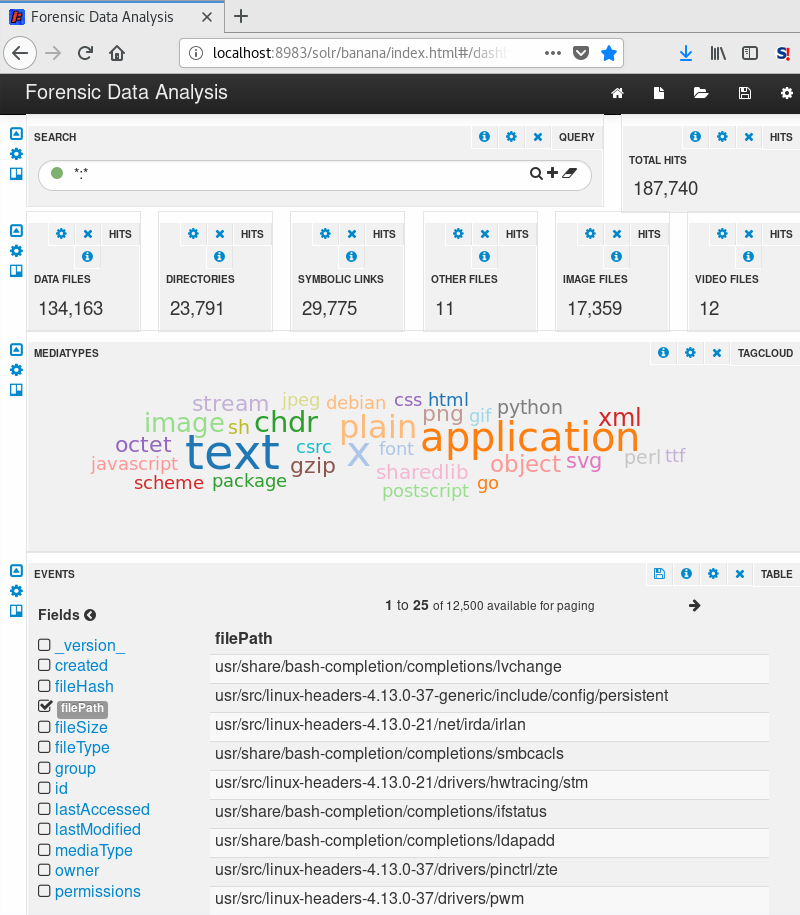
\includegraphics[width=\textwidth]{./resource/forensicDataAnalysisUI.png}
  \caption{Visualisierungsbeispiel mit Banana}
  \label{fig:banana_visualization}
\end{figure}

\noindent
Die UI selbst ist unterteilt in mehrere kleine Komponenten. Die erste Komponente ist die Volltextsuche, die es ermöglicht in den Metadaten nach bestimmten Wörtern und Werten zu suchen. In der zweiten Zeile befinden sich diverse Statistiken, die bei jeder Filterung oder Suche aktualisiert werden. Derzeit werden beispielsweise alle importierten Daten angezeigt. Dies sind insgesamt 187.740 Dateien. Darunter sind 134.163 Datendateien und 23.791 Verzeichnisse. In den Daten wurden 17.359 Bilder und 12 Videos erkannt. Diese Werte basieren auf der Datenauswertung der Medientypen, welche in bei der Datenverarbeitung ermittelt wurden (siehe Kapitel \ref{subsec:media_types}).
In der dritten Zeile werden die 30 häufigsten vorkommenden Medientypen in einer sogenannten \textit{Word Cloud} angezeigt. In der vierten Zeile hingegen werden die Ergebnisse der Suchanfrage angezeigt. Im konkreten Fall werden einfach die ersten beliebigen Dateien angezeigt. Sobald der Analyst aber beispielsweise nach einem bestimmten Dateinamen sucht, werden alle Dateien mit diesem Namen in der Ergebnissliste ausgegeben. Zusätzlich können einzelne Attribute visualisiert werden.\\
Es wäre auch möglich mit Banana eine Zeitleiste zu erstellen, um eine Filterung nach den Dateizeitstempel anzubieten.\\

\noindent
Gerade auch im Open-Source Bereich existieren noch weitere Projekte, welche zukünftig für eine Datenvisualisierung genutzt werden könnten. So wäre es möglich komplexe Zusammenhängen in der Graphendatenbank \textit{Neo4j} zu speichern und deren Graphenvisualisierung in die Web-Applikation zu integrieren.\footnote{Siehe Link: \url{https://neo4j.com/}. Letzter Zugriff: 24.9.2018.} Zur Erstellung weiterer Datenvisualisierungen könnten auch die Projekte \textit{Grafana}\footnote{Siehe Link: \url{https://github.com/grafana/grafana}. Letzter Zugriff: 24.9.2018.} oder \textit{Apache Superset}\footnote{Siehe Link: \url{https://github.com/apache/incubator-superset}. Letzter Zugriff: 24.9.2018.} genutzt werden.\\
Auch die JavaScript Bibliothek \textit{D3.js} bietet dutzende Arten zur Datenvisualisierungen, welche im forensischen Umfeld bei großen Datenmengen genutzt werden könnten.\footnote{Siehe Link: \url{https://d3js.org/}. Letzter Zugriff: 24.9.2018.}\\


% Wordcloud, geographische Visualisierung, Flare-Chart, Tree-Map, Calendar-Chart als Timeline?
% Webframeworks wie \url{https://d3js.org/} \footnote{Siehe Links: \url{https://bl.ocks.org/mbostock/4063550}, \url{https://bl.ocks.org/mbostock/5944371}, \url{https://bl.ocks.org/mbostock/1046712}, \url{https://bl.ocks.org/mbostock/4063269} und \url{http://xliberation.com/googlecharts/d3concept.html}. Letzter Zugriff: 25.7.2018}
% Open Source Community Variante Helical Insight
% Apache Superset für Visualisierung (siehe Ambari Cluster Services)
% Apache Grafana?
% GoJs incremental tree?
% Druid.io

%Duplicate Flag in DB schreiben, um über Banana UI alle Duplikate finden zu können...